% Chapter Template

\chapter{Engineering Demonstration} % Main chapter title

\label{ch:mammoth} % Change X to a consecutive number; for referencing this chapter elsewhere, use \ref{ChapterX}

\lhead{Chapter 5. \emph{Engineering Demonstration}} % Change X to a consecutive number; this is for the header on each page - perhaps a shortened title

%----------------------------------------------------------------------------------------
%	SECTION: INTRO
%----------------------------------------------------------------------------------------

\section{Introduction}
While analytic models provide insight to the operation of stochastic collocation for generalized polynomial chaos and high-density
model reduction methods, we are chiefly interested in applying these methods to engineering applications that lead to
decision making in real-world activities.  To this end, we selected multiphysics simulation code \mammoth{}, a \moose{}-based
\emph{MultiApp} that couples neutronics code \rattlesnake{}, fuel performance code \bison{}, and thermal hydraulics code
\texttt{relap-7}.  \mammoth{} solves these three sets of physics nonlinearly using picard iterations to feed back values until
convergence is achieved.

\section{Problem}
The model we selected is a two-dimensional slice of a pressurized water reactor fuel pin, including the fuel, gap, clad, and
moderator.  The fuel is separated into 23 axial rings, each with the same material properties but independent input uncertainty.
The response value of interest is the neutronics multiplication factor $k$-effective.  The model is documented
in \cite{physormammoth}.

TODO how many groups, etc.  Or should that go in the MODELS chapter?

The uncertain inputs are group-, burnup-, and temperature-dependent cross sections, as well as three \bison{}
inputs: fuel thermal expansion coefficient, fuel conductivity, and clad conductivity.
The macroscopic cross sections are calculated using \texttt{Scale} \cite{scale} along with a covariance matrix which provides
the correlation between cross sections.  Karhunen-Loevre \cite{karhunen} is used to decouple the resulting 671 inputs and
reduce them to 20 representative independent inputs.  This reduction is informed using \raven{} algorithms
considering both the KL expansion as well as input-output sensitivity, together referred to as the
\emph{importance rank}.  The cutoff was selected to \ldots TODO to MODELS chapter?

The simulation only considers neutronics (\rattlesnake{}) and fuel performance (\bison{}), so the thermal hydraulics is neglected.
The feedback from \rattlesnake{} to \bison{} is the power shape, and the feedback from \bison{} to \rattlesnake{} is the
temperature, which in turn affects the cross sections.  For performance, the number of Picard iterations
between the separate models
is limited to 6 per time step.  

TODO time steps, other input parameters, input file in appendix?, commit of MAMMOTH used

\moose{} and its applications including \rattlesnake{}, \bison{}, and \mammoth{} do not generally have a
versioning system or release
schedule; instead, it is tracked by \texttt{Git} \cite{git} commit hashes.
This computation was performed with the application versions listed in Table \ref{tab:git}.  There is nothing
particularly special about these versions, except that they were concurrent and compatible at the time
calculations were begun.
\begin{table}
  \centering
  \begin{tabular}{c c}
    App & Git Version Hash \\ \hline
    \moose{ } & 1fea13a34357a56c6fd049a239e57d597b1c277e\\
    \bison{ } & 5552eca741fa30be0efdefd35fecd954b47c9586\\
    \rattlesnake{ } & 2c892fad29ed7d1f7fb9833116d2b718f7b72055\\
    \mammoth{ } & be676b5974f990a0d2a7589ab2a2e58163a47b22 \\ \hline
    \raven{ } & 8f7c477740a8277c536d9bd6734614615a8b5cb7
  \end{tabular}
  \caption{Application Versions Used}
  \label{tab:git}
\end{table}

\section{Limitations}
During the collection of data, it was discovered that the performance of \bison{} can fluctuate depending on
the way is is parallelized.  There were instances where \bison{} would fail to converge, but report an unconverged
temperature as a converged solution.  As a result, there is artifical numerical error that is difficult to track or
account for.  Regardless, we demonstrate the performance of various methods on this model, as this behavior indicates
true simulation behavior.

\section{Results}
Figures \ref{fig:mammoth mean} and \ref{fig:mammoth var} show the values obtained for the mean and variance of
this model for a selection of uncertainty quantification methods, including
traditional Monte Carlo (\texttt{mc}),
static stochastic collocation for generalized polynomial chaos expansion using the total degree polynomial
construction indices (\texttt{td}), 
first- and second-order static Sobol decomposition (or HDMR) (\texttt{sobol}),
and adaptive Sobol decomposition using both adaptive cut-HDMR and adaptive generalized polynomial chaos
(\texttt{adaptSobol}).  For additional clarity, we provide graphs centered more especially on the non-Monte
Carlo data in Figures \ref{fig:mammoth mean zoom} and \ref{fig:mammoth var zoom}.  Because the number of Monte
Carlo runs necessary to obtain a well-resolved benchmark is prohibitive, we do not present any error
convergence plots for this model.

Table \ref{tab:mammoth
runs} summarizes the number of calculations required for each collocation method.  Entries marked with a
$\dagger$ indicate results that were not obtained because of \mammoth{} simulations that failed to converge.
Entries marked with a $*$ indicate results that were not attempted because of the number of samples required.
We note that in Table \ref{tab:mammoth} for first-order static Sobol method successive runs have the same
number of evaluations required despite constructing higher-order polynomials.  This is because we enforced a
floor function for quadrature, requiring a minimum number of quadrature points for a polynomial despite its
low order.  This
artificially increases the points for odd-numbered sets for this particular method, but prevents abnormally
poor integration.
\begin{table}
  \centering
  \begin{tabular}{c c|c}
    Method & Degree & Runs \\ \hline
    Total Degree & 1 & 47 \\
    Total Degree & 2 & 1105 \\
    Total Degree$^*$ & 3 & 17389 \\ \hline
    Sobol (1) & 1 & 47 \\
    Sobol (1) & 2 & 47 \\
    Sobol (1) & 3 & 93 \\
    Sobol (1) & 4 & 93 \\
    Sobol (1) & 5 & 139\\ \hline
    Sobol (2) & 1 & 47 \\
    Sobol (2) & 2 & 1105 \\
    Sobol (2)$^\dagger$ & 3 & 3221 \\
    Sobol (2)$^\dagger$ & 4 & 7361 \\
    Sobol (2)$^*$ & 5 & 13571 \\
  \end{tabular}
  \caption{Evaluations Required for 23 Input Pin Cell Model}
  \label{tab:mammoth}
\end{table}

We note that for both the mean and the variance, the collocation-based methods all converge within the
estimated Monte Carlo value single-standard deviation band with only first-order results.  This suggests a
high degree of linearity in the response.  In both the mean and the standard deviation, there appears to be
some convergence towards increasing the magnitude from the first-order expansions, but without a near-analytic
benchmark it is difficult to be certain if this is convergence to the true solution.  TODO more comments on
this?  Comment on how Sobol2 matches TD, and how that suggests linearity in the second-order interactions.
\begin{figure}[htb]
  \centering
  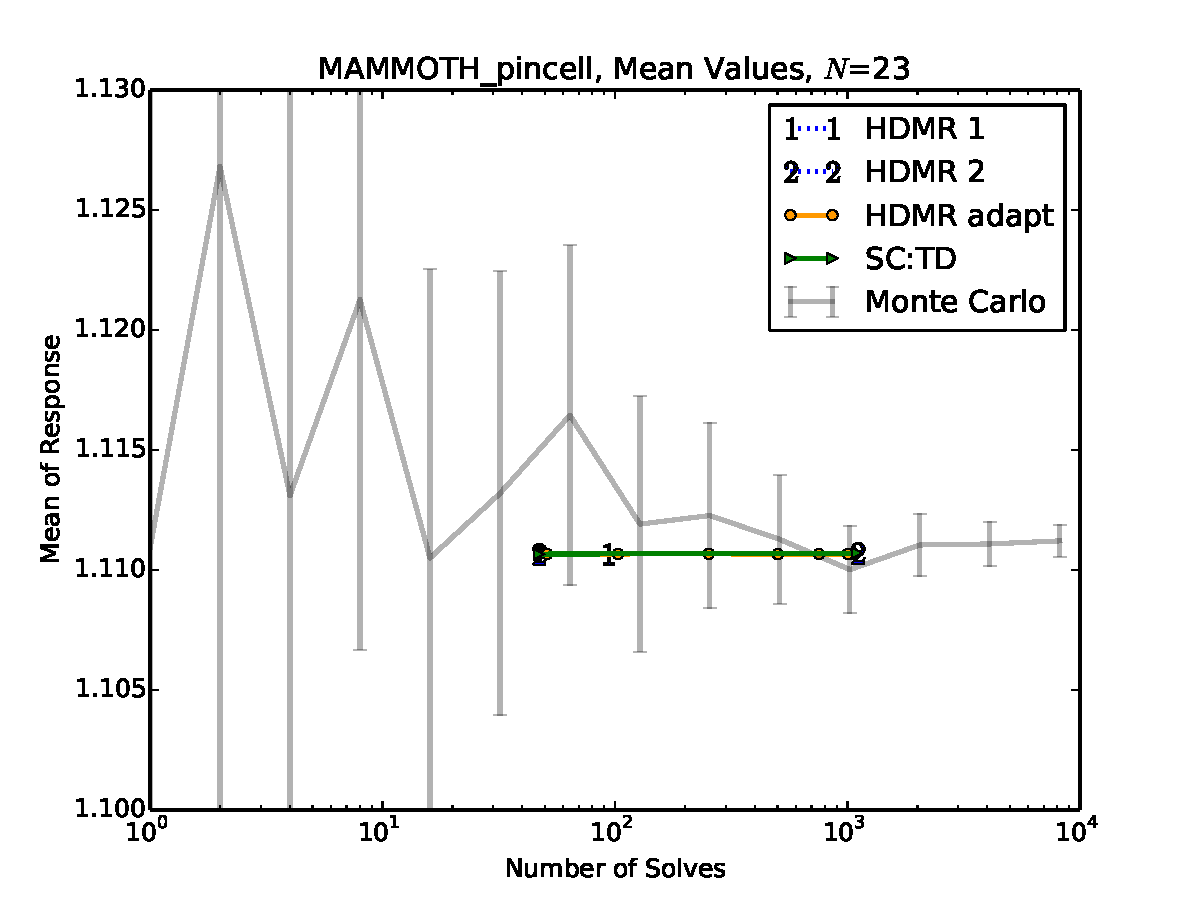
\includegraphics[width=0.7\linewidth]{mammoth/MAMMOTH_pincell_mean_vals}
  \caption{MAMMOTH Pin Cell, Mean Values}
  \label{fig:mammoth mean}
\end{figure}
\begin{figure}[htb]
  \centering
  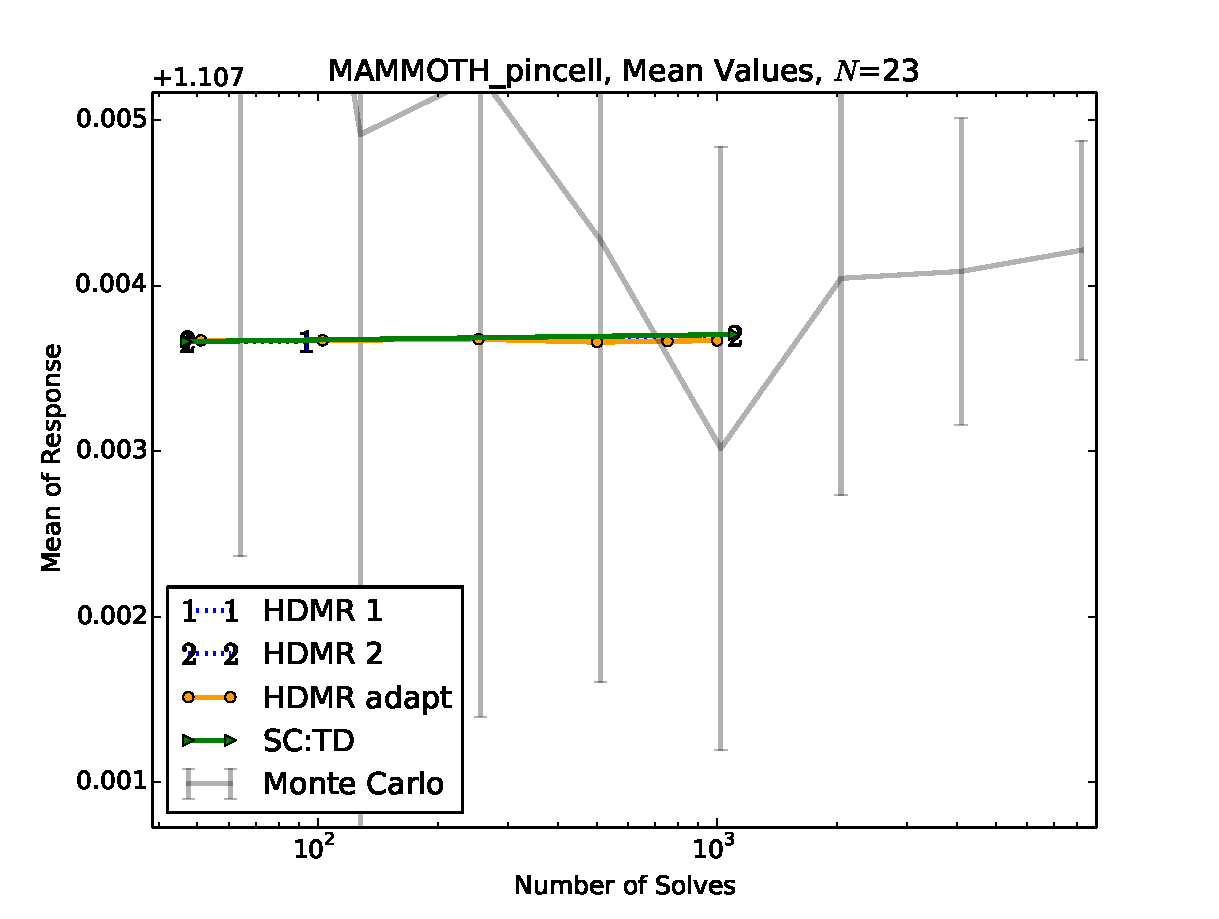
\includegraphics[width=0.7\linewidth]{mammoth/MAMMOTH_pincell_mean_zoom}
  \caption{MAMMOTH Pin Cell, Mean Values (Zoomed)}
  \label{fig:mammoth mean zoom}
\end{figure}
\begin{figure}[htb]
  \centering
  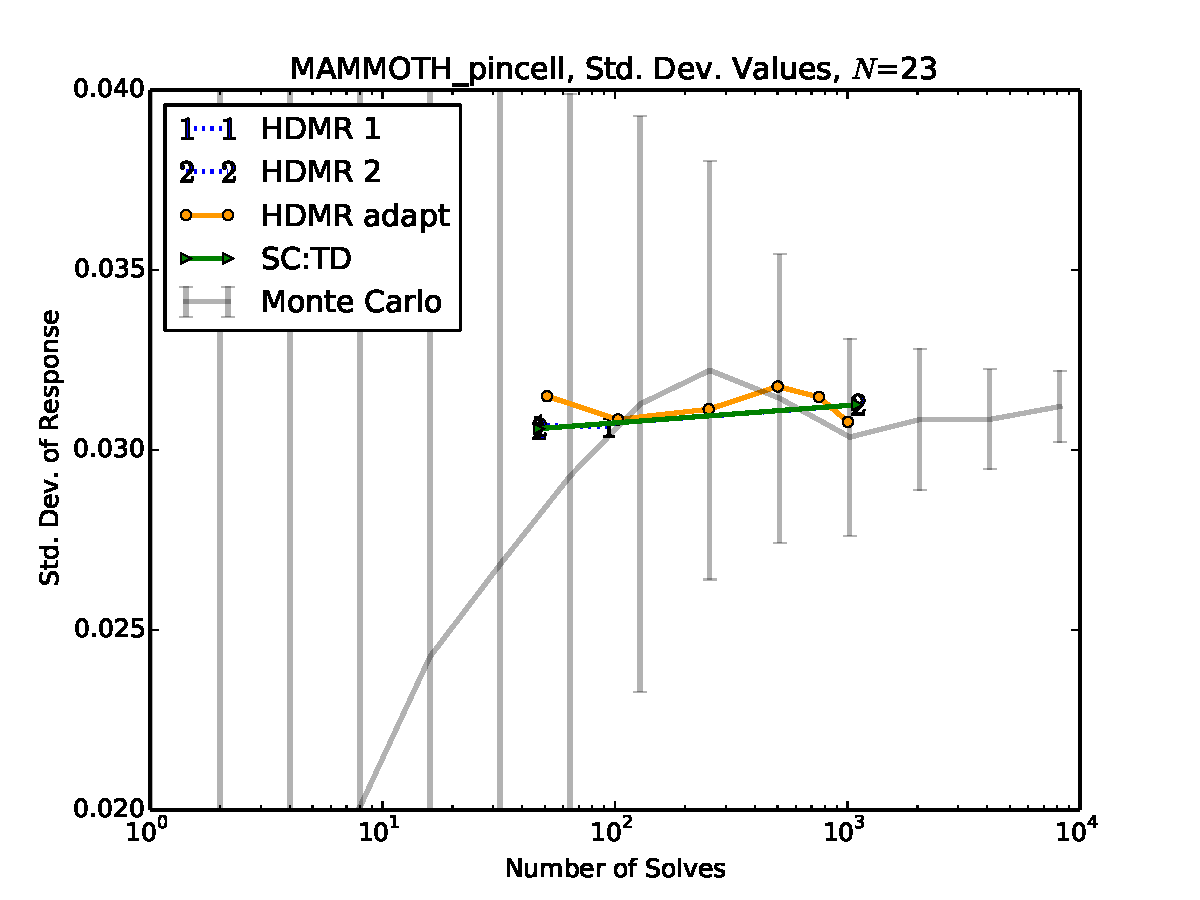
\includegraphics[width=0.7\linewidth]{mammoth/MAMMOTH_pincell_var_vals}
  \caption{MAMMOTH Pin Cell, Variance Values}
  \label{fig:mammoth var}
\end{figure}
\begin{figure}[htb]
  \centering
  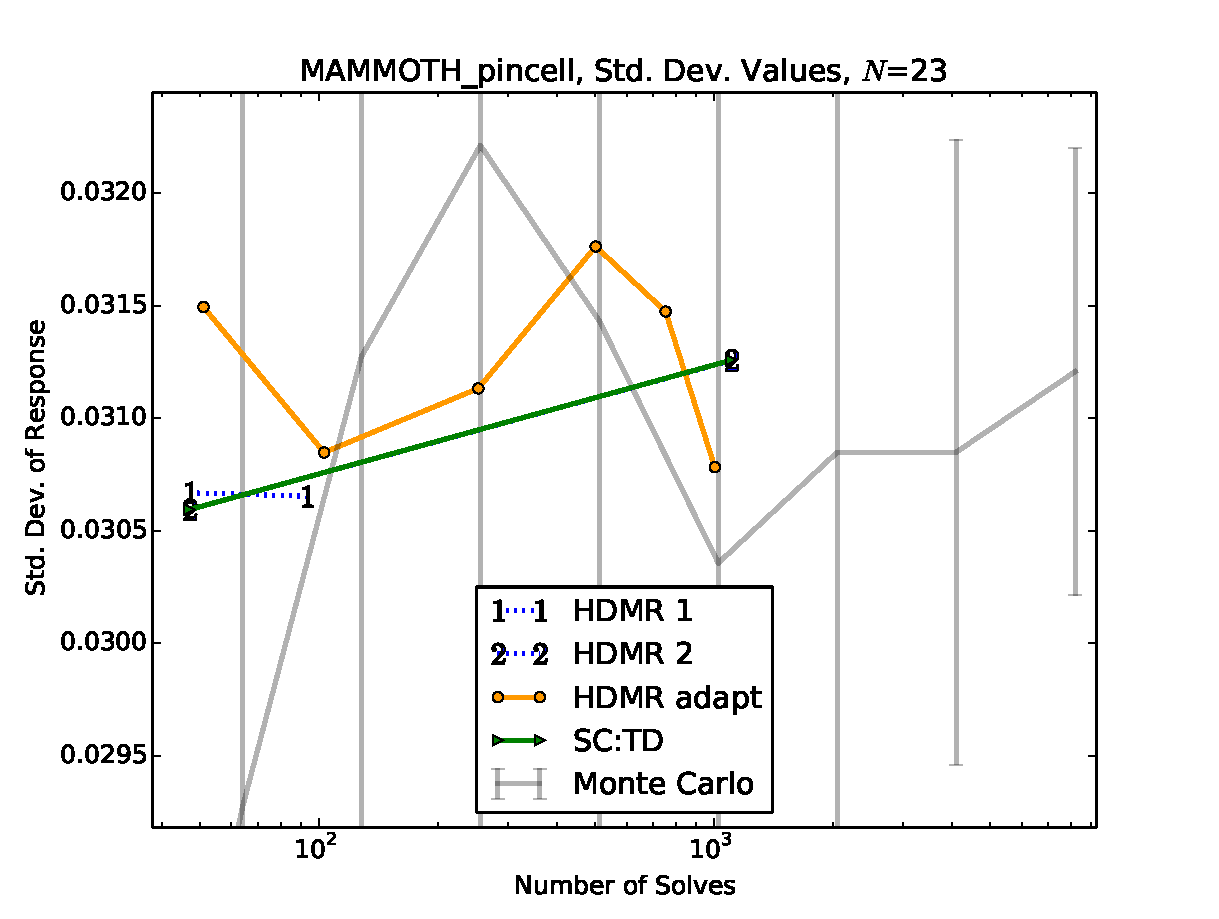
\includegraphics[width=0.7\linewidth]{mammoth/MAMMOTH_pincell_var_zoom}
  \caption{MAMMOTH Pin Cell, Variance Values (Zoomed)}
  \label{fig:mammoth var zoom}
\end{figure}

\section{Conclusions}
While the lack of an analytic benchmark makes it difficult to be certain how much better the collocation-based
methods are performing than traditional Monte Carlo, it is clear they are no worse even with first-order
approximations.  Additionally, with these first-order approximations only requiring roughly 47 evaluations
instead of ten thousand, we are prepared to conclude that all the collocation-based methods considered here
are more efficient for this model than traditional analog Monte Carlo when it comes to determining
second-order statistics.

%Run times
%
%For Picard 6 and SN (3 azimuthal, 3 polar Gauss Chebyshev):
%
%MPI 24: 11m 29.452s = 689.452 sec =  16546.848 single equivalent (0.424 efficient)
%MPI 12: 19m 41.703s = 1181.703 sec = 14180.436 single equivalent (0.495 efficient)
%MPI  6: 27m 50.373s = 1670.373 sec = 10022.238 single equivalent (0.701 efficient)
%MPI  1: 117m 0.756s = 7020.756 sec =  7020.756 single equivalent (1.000 efficient)
